\documentclass{hw-template}

\title{NE511 Homework 2}
\author{Kyle Hansen}
\date{10 March 2026}

\usepackage{cancel}

\renewcommand{\defeq}{\stackrel{\text{def}}{=}}



\begin{document}

\maketitle{}


\section{Analytical and Approximate Solutions to Point Kinetics}

The approximate and analytic solutions of the PKE are displayed in \autoref{fig:comparison}. 

The approximation assumes that:

\begin{enumerate}
    \item\label{item:a} $\rho < \beta /2$
    \item\label{item:b} $\Lambda \lambda \ll \beta$
    \item\label{item:c} $\Lambda \lambda \ll \rho$.
\end{enumerate}

All three conditions are only satisfied for Cases 1 and 2-- Case 3 does not satisfy \autoref{item:a}, and Case 4 does not satisfy \autoref{item:c}, so those cases are seen to be approximated poorly by the approximations in \autoref{fig:comparison}. Note that this may not be seen immediately in Case 3, since $\rho$ is higher than the other cases. Higher $\rho$ means that this configuration's time scale is much shorter than the other cases.



\begin{figure}
    \centering
    \begin{subfigure}{0.48\linewidth}
        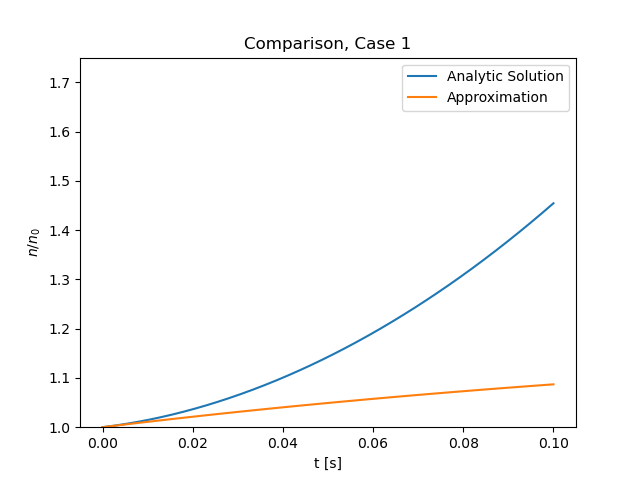
\includegraphics[width=\linewidth]{case1.png}
        \caption{Case 1}
    \end{subfigure}
    \begin{subfigure}{0.48\linewidth}
        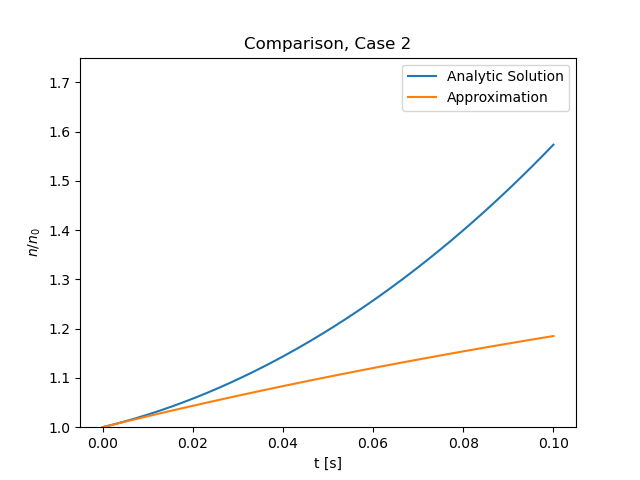
\includegraphics[width=\linewidth]{case2.png}
        \caption{Case 2}
    \end{subfigure}

    \begin{subfigure}{0.48\linewidth}
        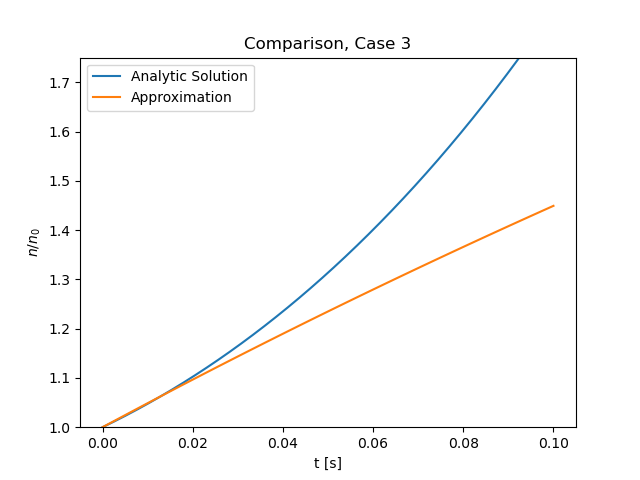
\includegraphics[width=\linewidth]{case3.png}
        \caption{Case 3}
    \end{subfigure}
    \begin{subfigure}{0.48\linewidth}
        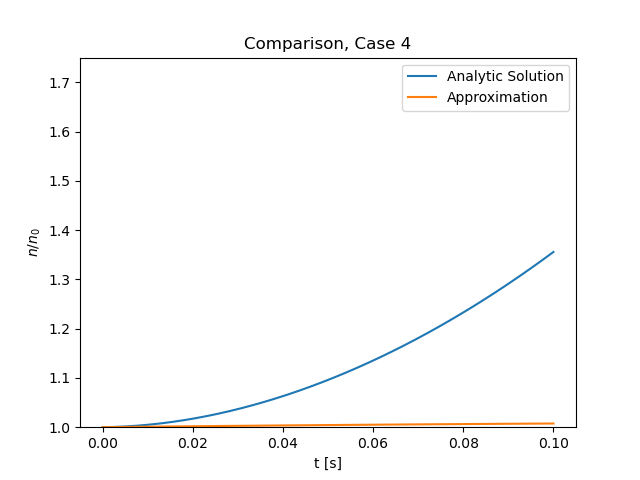
\includegraphics[width=\linewidth]{case4.png}
        \caption{Case 4}
    \end{subfigure}
    \caption{Comparision of Analytic and Approximate Solutions}\label{fig:comparison}
\end{figure}


\section{Super-prompt critical transient with energy feedback}\label{sec:second}

The burst width of this transient is

\begin{equation}
   \overline{\Delta}t =  \frac{4 \Lambda}{\rho_{p1}} \left(1 - \frac{p^0}{p_m} \right).
\end{equation}

With the given data, $\rho_{p1} = \rho_1 - \beta = 0.1\beta$, or $\rho_{p1} = 0.00075$, so

\begin{equation}
    \overline{\Delta}t \approx \frac{4 \cdot 10^{-5} \text{ s}}{0.00075} = 0.0533 \text{ s},
\end{equation}

or less, if the power jump is very large. The energy deposition is

\begin{equation}
    Q(t_2) = \frac{-2\rho_{p1}}{\gamma_e},
\end{equation}

which, assuming $\gamma \approx -0.8\$/\text{fp-s}$ (Ott), leads to 

\begin{equation}
    Q(t_2) = \frac{2 \cdot 0.1}{0.8} = 0.25 \text{fp-s},
\end{equation}

which is about 4.69 times the typical energy produced in that time.

\subsection{} If heat release is neglected, the calculated temperature in the fuel is higher than in reality, leding to a shorter-than-physical burst and a lower-than-physical total energy deposition $Q$, though the discrepancy is likely small for the given configuration.

\subsection{} $P_0$ is a source of energy (raises temperature), so neglecting this leads to a longer-than-physical calculated burst width and higher-than-physical burst energy deposition.

\section{Sub-prompt critical reactivity step insertion}

In the case that Doppler feedback exactly balances delayed neutrons,

\begin{equation}
    p^{00} = \frac{-\beta \overline{\lambda}}{\gamma}.
\end{equation}

Then the U-235 power is

\begin{equation}
    p^{00}_U = \frac{0.4 \text{ s}^{-1}}{0.16 \text{ \$/fp/s}} = 2.5 \text{ fp}
\end{equation}

and the MOX power is

\begin{equation}
    p^{00}_{mox} = \frac{0.6 \text{ s}^{-1}}{0.08 \text{ \$/fp/s}} = 7.5 \text{ fp}.
\end{equation}

The main driver in the difference between these values is is the feebdack coefficient:the MOX reactor has a much lower Doppler coefficient (the cross sections change less given the same temperature change), so the reactivity decreases much more slowly, and there is more time for the power to increase.

\section{Power amplitude evolution}

First, since $\rho_{p1} = 0.1$, and 

\begin{equation}
    \rho_b = \sqrt{\rho_{p1}^2 - 2 \Lambda \gamma p^0},
\end{equation}

then using $p^0 = 1$,

\begin{equation}
    \rho_b = \sqrt{0.1^2 - 2 \left( \frac{1 \text{ s \$}^{-1}}{0.62 \times 10^4} \right) \left( -0.08 \text{ \$ fp}^{-1}\text{s}^{-1} \right)} = 1.001289, 
\end{equation}

and maximum power is

\begin{equation}
    p_m = -\frac{\rho_b^2}{2 \Lambda \gamma} = \frac{0.0100258}{2 \cdot (0.62 \times 10^4)^{-1} \cdot 0.08} \text{ fp} = 388.5 \text{ fp} .
\end{equation}

Using these parameters, the pulse can be plotted, and is show in \autoref{fig:last}.


\begin{figure}
    \centering
    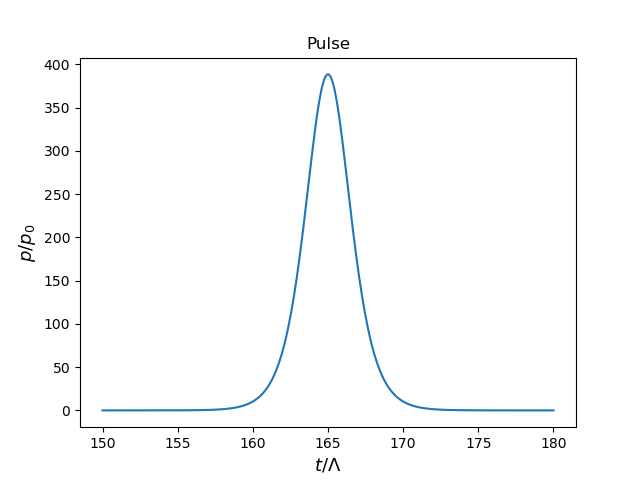
\includegraphics[width=0.65\textwidth]{pulse.png}
    \caption{Power jump following super-prompt critical step insertion}\label{fig:last}
\end{figure}

In this model, with no energy loss (as in Question 2) and linear energy feedback, the pulse is symmetric about $t_m$. One of the most important features is that the pulse width is proportional to $\Lambda$ and the pulse height is proportional to $1/\Lambda$.


\end{document}
